% Vorlage_Qualifikationsarbeit_Thesis.tex


\documentclass[
  paper=a4, % DIN-A4-Format
  11pt, % Schriftgröße
  bibliography=totoc, % Bibliografie automatisch im Inhaltsverzeichnis generieren
  parskip=off, % Absatzabstand: off, half, full
  oneside, % einseitiges Layout
%  twoside, % zweiseitiges Layout
  article, % verwendet KOMA-Klasse scrartcl
%  longdoc=true,
  accentcolor=tud8b, % tud9a usw.
%  colorbacktitle, % Hintergrund des Titels einfärben
  colorback, % Hintergrund unter dem Titel einfärben
  type=dr, % für eingereichte Dissertationen
%  type=drfinal, % für genehmigte Dissertationen
  dr=ing % Titel: ing, rernat, phil
]{tudthesis}


% INFO %
% Im Folgenden die Pakete, die diese Vorlage lädt.
% Informationen über eine Vielzahl von Paketen gibt es auf CTAN (Comprehensive TeX Archive Network)
% http://ctan.org/

\usepackage[T1]{fontenc}
\usepackage[utf8]{inputenc} % korrekte Darstellung von Umlauten u. Sonderzeichen
\usepackage[ngerman]{babel} % Sprachpaket, ngerman = neue deutsche Rechtschreibung
\usepackage[stable]{footmisc} % mehr Optionen für Fußnoten
\usepackage{booktabs} % hübschere Tabellen als der LaTeX-Standard
\usepackage{multirow} % Create tabular cells spanning multiple rows
\usepackage{longtable} % große Tabellen, die sich über mehrere Seiten erstrecken
\usepackage{listings} % bietet Umgebung, um Programmiercode zu setzen inkl. Syntaxhighlighting
\usepackage{amsmath} % Setzen mathematischer Formeln
\usepackage{ellipsis} % korrigiert Aussehen von „…“
\usepackage{enumitem} % mehr Optionen für Aufzählungen
\usepackage[shortcuts]{extdash} % mehr Optionen für Worttrennung
\usepackage{setspace} % Zeilenabstände verändern: \singlespacing, \onehalfspacing oder \doublespacing
\usepackage{lipsum} % zur Erzeugung von Lorem-Ipsum-Blindtext
\usepackage[math]{blindtext} % zur Erzeugung von deutschem Blindtext
\usepackage{hyperref} % Verlinkungen im Dokument

% INFO %
% Das hyperref-Paket sollte möglichst als letztes geladen werden, darum steht es weiter hinten in der Präambel.
% Leider funktioniert hyperref nicht 100%-ig einwandfrei mit tudstyle; bei Problemen damit lieber aus dem Dokument entfernen!

% Einstellungen für hyperref
\hypersetup{%
    pdftitle=Meine Dissertation,
    pdfauthor=Greta Lund,
    pdfsubject=Dissertation,
    unicode=true, % benötigt, damit Umlaute im pdftitle richtig dargestellt werden
    breaklinks=true
    %% colorlinks=true
    %% linkcolor=NavyBlue,
    %% urlcolor=NavyBlue,%Green4,
    %% citecolor=NavyBlue%DeepPink3
}


%%%%%%%%%%%%
% BibLaTeX %
%%%%%%%%%%%%

% INFO %
%
% Bibliografien mit LaTeX
%
% biblatex ist eine komplette moderne Neuentwicklung von bibtex, u.a. mit vollständiger Unterstützung von UTF-8.
%
% Ausführliche Dokumentation und Nutzungshandbuch: http://mirrors.ctan.org/macros/latex/contrib/biblatex/doc/biblatex.pdf
%
% Für geisteswissenschaftliche Arbeiten sind die Biblatex-Stile von Dominik Waßenhoven zu empfehlen:
% http://biblatex.dominik-wassenhoven.de


\usepackage[
    backend=biber, % biber ist das Standard-Backend für Biblatex. Für die Abwärtskompatibilität kann hier auch bibtex oder bibtex8 gewählt werden (siehe biblatex-Dokumentation)
    style=authortitle, %numeric, authortitle, alphabetic etc.
    autocite=footnote, % Stil, der mit \autocite verwendet wird
    sorting=nty, % Sortierung: nty = name title year, nyt = name year title u.a.
    sortcase=false,
    url=false,
    hyperref=auto,
]{biblatex}



\renewbibmacro*{cite:seenote}{} % um zu verhindern, dass in Fußnoten automatisch "(wie Anm. xy)" eingefügt wird
\DeclareFieldFormat*{citetitle}{\mkbibemph{#1\isdot}} % zitierte Titel kursiv formatieren
\DeclareFieldFormat*{title}{\mkbibemph{#1\isdot}} % zitierte Titel kursiv formatieren

\addbibresource{Literaturverzeichnis.bib} % Hier Pfad zu deiner .bib-Datei hineinschreiben
\nocite{*} % Alle Einträge in der .bib-Datei im Literaturverzeichnis ausgeben, auch wenn sie nicht im Text zitiert werden. Gut zum Testen der .bib-Datei, sollte aber nicht generell verwendet werden. Stattdessen lieber gezielt Einträge mit Keywords ausgeben lassen (siehe \printbibliography in Zeile 224).


% INFO %
% Hier kannst du deine persönlichen Daten hineinschreiben und diese Variablen verwenden, damit du es nicht jedes Mal neu schreiben musst.

\newcommand*{\myname}{Greta Lund}
\newcommand*{\mytitlede}{Meine Dissertation: Fragen und Antworten}
\newcommand*{\mytitleen}{My Thesis: Questions and Answers}
\newcommand*{\mymail}{\href{mailto:gretalund@example.com}{gretalund@example.com}}
\newcommand*{\myprof}{Prof. Dr. Patricia Davis}
\newcommand*{\myinstitute}{Gruppe Verteilte Systeme}
\newcommand*{\myfaculty}{Fachbereich Informatik}



%%%%%%%%%%%%%%%%%%%%%%%%%%%%%%%%%%%%%%%%%%%%%%%%%%%%%%%%%%%%%%%%%%%%%%%%%%%%%%%%



\begin{document}

\parindent 0em % Erstzeileneinzug


% Titelei

\author{\myname}
\thesistitle{\mytitlede}{\mytitleen}
\birthplace{Kopenhagen}
\date{4.2.2016}
\referee{\myprof}{Dr.~Michael Brown}
\department{\myinstitute}
\group{\myfaculty}
\dateofexam{17.5.2016}{4.2.2016}
\makethesistitle

% Eigenständigkeitserklärung: muss nach \makethesistitle erscheinen, sonst wird sie als erste Seite des Dokuments gesetzt.
\affidavit[4.2.2016]{\myname}
%\affidavit{\myname}


\pagestyle{myheadings} % Seitenstil umschalten
\mymarkright{Version: \today} % Inhalt der Fußzeile


% Abstract bzw. Zusammenfassung der Arbeit
% INFO
% Abstract.tex
% Für den Abstract der Abschlussarbeit oder Dissertation

\begin{abstract}
  Dies ist der Abstract der Arbeit.
  Er gibt wertungsfrei, kurz und prägnant den Inhalt der wissenschaftlichen Arbeit wieder.
\end{abstract}  


\clearpage

%\pagenumbering{Roman} % Seitennummerierung auf römische Zahlen ändern

\setcounter{tocdepth}{3}
\tableofcontents % Inhaltsverzeichnis
\setcounter{page}{1}
\clearpage



% Aktuelle Seitenzahl speichern, da Wechsel auf arabische Zahlen die Zählung zurücksetzt
%% \newcounter{savedromanpagenumber}
%% \setcounter{savedromanpagenumber}{\value{page}}
%\pagenumbering{arabic} % Arabische Seitenzahlen


% Im Folgenden eine beispielhafte Gliederung mit Blindtext, Formeln, Tabellen und Bildern, die du an deinen Bedarf anpassen kannst.

\section{Einleitung}
\parindent 2em
\onehalfspacing

Dieses Dokument zeigt, wie eine Dissertation oder Abschlussarbeit in {\LaTeX} an der TU Darmstadt aussehen kann.
Es enthält Abschnitte und Unterabschnitte für eine beispielhafte Dokumentstruktur und illustriert den Gebrauch von Tabellen, Formeln und Abbildungen.


\clearpage


\section{Kriterien guter Arbeiten}

Dies hier ist ein Blindtext zum Testen von Textausgaben. Wer diesen Text liest, ist selbst schuld. Der Text gibt lediglich den Grauwert der Schrift an.\autocite[668]{Tanenbaum2008}
Ein Blindtext sollte möglichst viele verschiedene Buchstaben enthalten und in der Originalsprache gesetzt sein. Er muss keinen Sinn ergeben, sollte aber lesbar sein.\autocite[43]{Schill2012}

\subsection{Wissenschaftliche Lauterkeit}
\blindtext

\paragraph{Ein Abschnitt}
\blindtext

\paragraph{Noch ein Abschnitt}
\blindtext


\subsection{Sichere Anwendung von Methoden}
\Blindtext

\subsection{Einheitliches Erscheinungsbild}
\blindtext

\clearpage



\section{Grafische Elemente}

\subsection{Tabellen}
% Tabelle.tex

Dies ist ein Beispiel für eine Tabelle, die mit dem Paket „booktabs“\footnote{Nähere Informationen über das Paket sind auf CTAN zu finden: \url{http://ctan.org/pkg/booktabs}.} erstellt wurde.

\vspace{0.5em}

\begin{center}
%\sffamily

\begin{tabular}{rlr}\toprule
Nr. & Bezeichnung & Zahl \\
\midrule
90 & Bachelor & 39,40 \\
443 & Diplom & 272,00 \\
6667 & Dissertation & 0,39 \\
\bottomrule
\end{tabular}

\end{center}





\subsection{Mathematische Formeln}
% Formeln.tex

Berechnung der Fibonacci-Folge:

\begin{equation}
f_n = \frac{\varphi^n - \psi^n}{\varphi-\psi}, \qquad n \in \mathbb Z
\end{equation}

\noindent Berechnung der harmonischen Reihe:

\begin{equation}
H_n=\sum_{k=1}^n \frac{1}{k}=1 + \frac{1}{2} + \frac{1}{3} + \frac{1}{4} + \cdots +\frac{1}{n}
\end{equation}







\subsection{Abbildungen}
% Abbildungen.tex

% Quellenangabe: Das Bild der Kamille stammt von Wikimedia Commons und wurde von Simplicius erstellt.
% https://commons.wikimedia.org/wiki/File:Kamille_01.jpg

Dies ist eine Abbildung.

\begin{figure}[htb]
    \centering
    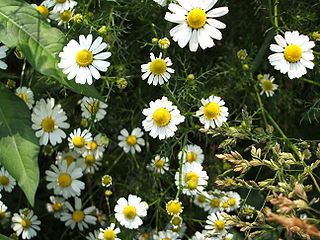
\includegraphics[height=6cm]{320px-Kamille_01.jpg}
    \caption{Kamillenblüte, \emph{Matricaria chamomilla}. Wikimedia Commons, Simplicius, \url{https://commons.wikimedia.org/wiki/File:Kamille_01.jpg}}
    \label{kamille}
\end{figure}





\clearpage


\section{Resümee}
\blindtext
%% \addsec{Ausblick}
%% \addsec{Schlusswort}

\clearpage


%%%%%%%%%%%%%%%%%%%%%%%%%%%%%%%%%%%%%%%%%%%%%%%%%%


% Bibliografie mit BibLaTeX
%
% Verwende keyword=meinbegriff, um nur die Einträge aus deiner .bib-Datei ausgeben zu lassen, die mit meinbegriff getaggt sind.
% Darf ein bestimmtes Keyword nicht enthalten sein, verwende notkeyword=meinbegriff.

\singlespacing
\printbibliography[title=Literaturverzeichnis, heading=bibliography]
%\printbibliography[title=Literaturverzeichnis, heading=bibliography, keyword=meinbegriff]

\clearpage


%%%%%%%%%%%%%%%%%%%%%%%%%%%%%%%%%%%%%%%%%%%%%%%%%%


% Beginn des Anhangs

\appendix

%% \pagenumbering{Roman}
%% \setcounter{page}{\value{savedromanpagenumber}+1} % gespeicherte Seitenzahl vom Beginn des Dokuments aufrufen und damit weiterzählen

\section{Abkürzungsverzeichnis}
\clearpage
\section{Transkription der Interviews}



\end{document}
